%--------------------------------------------------------------------------
%
%                                                    SOLUTION
%
%--------------------------------------------------------------------------

\begin{center}
\vspace*{5mm}
\noindent {\Large {\bf (Solution) }}
\end{center}


\begin{enumerate}
\item[a)] If we redefine the time origin as well as the space origin, we can always bring the equation of a harmonic oscillator back to $x(t)=A\sin(\omega t)$. In that form, the speed and acceleration are respectively $v(t)=A\omega \cos(\omega t)$ and $a(t)=-A\omega^2\sin(\omega t)$. We can then deduce that...
\begin{itemize}
\item ...the norm of the velocity is maximal at $\omega t=n\pi$ (where $n$ is an integer), that is, at the equilibrium position $x=0$.
\item ...the acceleration is naught at  $\omega t=n\pi$, that is, at the equilibrium position $x=0$.
\item ...the speed is naught at $\omega t=\pi/2+n\pi$, that is, at the extremal positions $x=\pm A$. 
\item ...the norm of the acceleration is maximal at $\omega t=\pi/2+n\pi$, that is, at the extremal positions $x=\pm A$. 
\end{itemize}
\item[b)] Yes, it is possible: for the speed to increase, the acceleration must be positive. It is, of course, possible for the acceleration to decrease while remaining positive. 
\begin{itemize}
\item Let's see the example of an object moving along the $x$ axis, whose acceleration decreases linearly as a function of time $a=a_0(1-\alpha t)$, $a_0>0$, $\alpha >0$. If we calculate the variation, between times $t$ and   $t+\Delta t$, of the acceleration and of the speed, we find :
$$\Delta a=a(t+\Delta t)-a(t)=a_0(1-\alpha(t+\Delta t))-a_0(1-\alpha t)=-a_0 \alpha \Delta t <0$$
$$
\Delta v=a_0 (1-\alpha t)\Delta t >0  
$$
Therefore, so long as $\alpha t<1$, the speed variation $\Delta v$ is positive even though the acceleration variation $\Delta a$ is negative.

\item For a more day-to-day example, imagine a cyclist on a downwards slope. She is pedalling at the beginning of the slope, but then stops to free-wheel down. When she is pedalling, her acceleration is greater than when she is free-wheeling; nevertheless, even then, her speed will keep increasing.
\item In harmonic oscillator motion, as shown in the following diagram for a $\pi/10$ pulsation, there are times, like between 15 and 20 s or between 35 and 40 s, when the acceleration decreases (green curve) while the speed increases (blue curve). This can be expressed analytically when we consider the motion $x(t)=A\sin(\omega t)$, of which the speed is $v(t)=\frac{dx}{dt}=A\omega\cos(\omega t)$, the acceleration is $a(t)=\frac{d^2x}{dt^2}=-A\omega^2\sin(\omega t)$, and the acceleration variation is $\frac{da}{dt}=-A\omega^3\cos(\omega t)$. The speed variation, then, is opposite in sign to the acceleration variation  $\frac{da}{dt}$ if $\pi/2<\omega <\pi$ or $3\pi/2<\omega<2\pi$.
\end{itemize}
\end{enumerate}
%\begin{center}\scalebox{0.6}{\input{serie02_concept.pdf_t}}\end{center}
\begin{center}
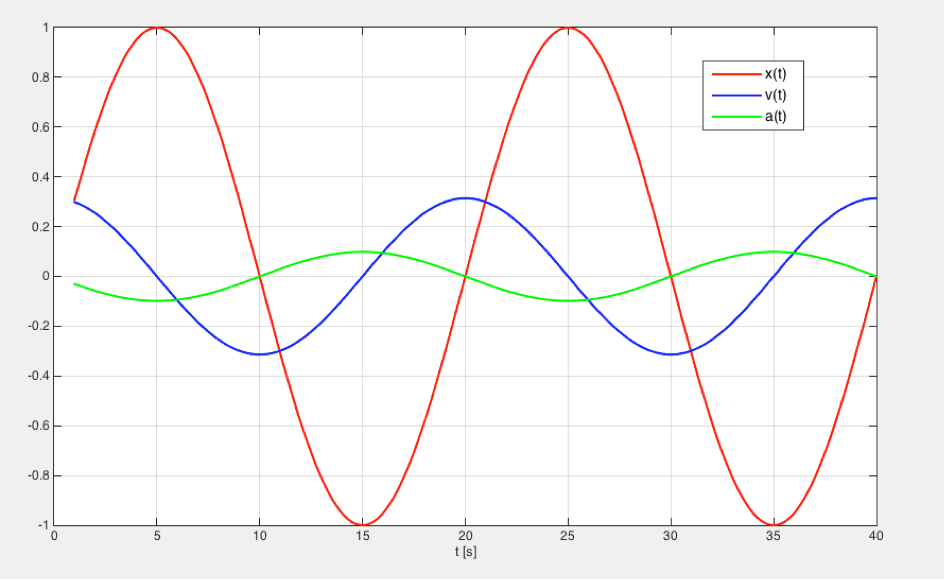
\includegraphics[width=.8\textwidth]{figures/serie02_concept.pdf}
\end{center}
